\documentclass[twocolumn,twoside,letterpaper]{article} 

\usepackage{color}

\usepackage{geneticsT2}
\usepackage{times}

\addtolength{\oddsidemargin}{-.2cm}
\addtolength{\evensidemargin}{-1.2cm}

\addtolength{\textwidth}{1.5cm}
\addtolength{\topmargin}{-2cm}
\addtolength{\textheight}{3.5cm}

\renewcommand{\textfraction}{0.01}
\renewcommand{\topfraction}{0.99}
\renewcommand{\bottomfraction}{0.65}
\renewcommand{\floatpagefraction}{0.90}
\renewcommand{\dbltopfraction}{0.95}
\renewcommand{\dblfloatpagefraction}{0.80}
\renewcommand{\sfdefault}{phv}

% plr added
\newcommand{\mutrate}{\lambda_{\text{mut}}}
\newcommand{\migrate}{\lambda_{\text{mig}}}
\newcommand{\Tmut}{T_{\text{mut}}}
\newcommand{\Tmig}{T_{\text{mig}}}

\usepackage{fancyhdr}
\pagestyle{fancy}
\fancyhf{}
%\fancyhead[LE,RO]{\thepage}
%\fancyhead[CE]{S. Takuno \emph{et al}.}
%\fancyhead[CO]{Pseudogene preservation by gene conversion}
\fancyfoot[LE,RO]{{\sfbf \thepage}}
\renewcommand{\headrulewidth}{0pt}
\fancypagestyle{plain}{
	\fancyhf{}
}

%editing commands (please leave in for now)
\newcommand{\jri}[1]{\textcolor{blue}{ \emph{\scriptsize  #1}} }
\newcommand{\st}[1]{\textcolor{red}{#1}}
\newcommand{\comst}[1]{\textcolor{red}{ \em{\scriptsize  #1}} }
\definecolor{mattgreen} {rgb} {0,0.6,0}
\newcommand{\mbh}[1]{\textcolor{mattgreen}{ \em{\scriptsize  #1}} }
\definecolor{peterpurple}{rgb}{.6,0,.6}
\newcommand{\plr}[1]{\textcolor{peterpurple}{ \emph{\scriptsize (#1)}} }

\usepackage[normalem]{ulem}
\def\dt{\bgroup
 \markoverwith{\lower-0.2ex\hbox
 {\kern-.03em\vbox{\hrule width.2em\kern0.45ex\hrule}\kern-.03em}}%
 \ULon}
\MakeRobust\dt
\usepackage[normalem]{ulem}
\def\dt{\bgroup
 \markoverwith{\lower-0.2ex\hbox
 {\kern-.03em\vbox{\hrule width.2em\kern0.45ex\hrule}\kern-.03em}}%
 \ULon}
\MakeRobust\dt

%%%%

\title{The molecular basis of parallel adaptation to\\ highland climate in domesticated maize}
\author{
 \small\sfbf{Shohei Takuno$^{\ast}$, Peter Ralph$^{\dag, \ddag}$, Sofiane Mezmouk$^{\ast}$, Kelly Swarts$^{\S}$, Rob J. Elshire$^{\S}$, Jeffrey C. Glaubitz$^{\S}$,}\\
   \small\sfbf{Edward S. Buckler$^{\S, \ast\ast}$, Matthew B. Hufford$^{\ast}$, and Jeffrey Ross-Ibarra$^{\ast,\dag\dag,}$}\thanks{
Corresponding author:  Department of Plant Sciences, University of California, Davis, California 95616, USA. 
    E-mail: \mbox{rossibarra@ucdavis.edu}}\\[0.3cm]
   \small\sf $^{\ast}$Department of Plant Sciences, University of California, Davis, California 95616, USA,\\
   \small\sf $^\dag$ Department of Evolution and Ecology, University of California, Davis, California 95616, USA,\\
   \small\sf $^\ddag$Department of Biological Sciences, University of Southern California,  Los Angeles,California 90089-0371, USA,\\
   \small\sf $^\S$Institute for Genomic Diversity, Cornell University, Ithaca, New York 14853-2703, USA,\\
   \small\sf $^{\ast\ast}$US Department of Agriculture�Agriculture Research Service (USDA-ARS) \st{address},\\
   \small\sf $^{\dag\dag}$The Center for Population Biology and the Genome Center, University of California, Davis, California 95616 , USA\\
}

 
\date{Revised manuscript for \emph{Genetics}, \today}

\abstract{
Parallel adaptation is defined as the independent evolution of multiple species/subpopulations to similar environments via adaptive mutations in the same locus.
We investigate here the molecular basis of maize adaptation to highland climates in Mexico and South America using genome-wide SNP data. 
Taking advantage of arachaeolgoical data on the arrival of maize to the highlands, we infer demographic models for both populations, identifying evidence of a strong bottleneck and rapid expansion in South America.  
We use these models to then identify loci showing an excess of differentiation as a means of identifying putative targets of natural selection, and compare our results to expectations from recently developed theory on parallel adaptation.  
In spite of similar morphologies, we see limited evidence of selection on quantitative traits, and, consistent with predictions across a wide array of paramater space, we see few SNPs showing signs of parallel adaptation.
%need to tweak this for Sofiane's GWAS
Instead, we show that selection appears to have prediminantly acted on standing genetic variation, and that introgression from wild teosinte populations appears to have played a role in adaptation in Mexican maize.
We discuss the significance of these results in the context of the molecular basis of adaptation to new environments. }

\usepackage{natbib}
\bibpunct{(}{)}{;}{a}{}{,}

\usepackage{amsmath}

\usepackage{graphicx}

\begin{document}

\maketitle

%%%%%%%%%%%%%%%%%%%%%%%%%%%%%%%%%%%%%%%%%% INTRO
\section*{Introduction}
\noindent Convergent evolution occurs when multiple species or populations exhibit similar phenotypic adaptations to comparable environmental challenges \cite[]{Wood_2005_15881688,Arendt_2008_18022278,Elmer_2011_21459472}.
Evolutionary genetic analysis of a wide range of species has provided evidence for multiple pathways of convergent evolution. 
One such route occurs when identical mutations arise independently and fix via natural selection in multiple populations. 
In humans, for example, malaria resistance due to mutations from Glu to Val at the sixth codon of the $\beta$-globin gene has arisen independently on multiple unique haplotypes  \cite[]{Currat_2002_11741197,Kwiatkowski_2005_16001361}.  
Convergent evolution can also be achieved when different mutations arise within the same locus yet produce similar phenotypic effects.  
Grain fragrance in rice appears to have evolved along these lines, as populations across East Asia have similar fragrances resulting from at least eight distinct loss-of-function alleles in the  \emph{BADH2} gene \cite[]{Kovach_2009_19706531}.  
Finally, convergent evolution may arise from natural selection acting on standing genetic variation in an ancestral population.  
In the three-spined stickleback, natural selection has repeatedly acted to reduce armor plating in independent colonizations of freshwater environments.  
Adaptation in these populations occurred both from new mutations as well as standing variation at the \emph{Eda} locus in marine populations \cite[]{Colosimo_2005_15790847}.  

Not all convergent phenotypic evolution is the result of convergent evolution at the molecular level, however.  
Recent studies of adaptation to high elevation in humans, for example, reveal that the genes involved in highland adaptation are largely distinct among Tibetan, Andean and Ethiopian populations \cite[]{Bigham_2010_20838600,Scheinfeldt_2012_22264333,Alkorta-Aranburu_2012_23236293}. 
While observations of independent origin may be due to a complex genetic architecture or standing genetic variation, introgression from related populations may also play a role.  
In Tibetan populations, the adaptive allele at the \emph{EPAS1} locus appears to have arisen via introgression from Denisovans, a related hominid group \cite[]{huerta2014altitude}.
Overall, we still know relatively little about how convergent phenotypic evolution is driven by common genetic changes or the relative frequencies of these different routes of convergent evolution.

The adaptation of maize to high elevation environments (\emph{Zea mays} ssp. \emph{mays}) provides an excellent opportunity to investigate the molecular basis of convergent evolution.  
Maize was domesticated from the wild teosinte \emph{Zea mays} ssp. \emph{parviglumis} (hereafter \emph{parviglumis}) in the lowlands of southwest Mexico $\sim$9,000 years before present (BP) \cite[]{Matsuoka_2002_11983901,Piperno_2009_19307570,vanHeerwaarden_2011_21189301}. 
After domestication, maize spread rapidly across the Americas, reaching the lowlands of South America and the high elevations of the Mexican Central Plateau by $\sim 6,000$ BP \cite[]{Piperno_2006_69}, and the Andean highlands by $\sim 4,000$ BP \cite[]{Perry_2006_16511492,Grobman_2012_22307642}. 
The transition from lowland to highland habitats spanned similar environmental gradients in Mesoamerica and S. America (Figure~\ref{supp:colfreq}) and presented a host of novel challenges that often accompany highland adaptation including reduced temperature, increased ultraviolet radiation, and reduced partial pressure of atmospheric gases \cite[]{Korner_2007_17988759}.

Common garden experiments in Mexico reveal that highland maize has successfully adapted to high elevation conditions \cite[]{Mercer2008}, and phenotypic comparisons between Mesoamerican and S. American populations are suggestive of convergent evolution.  
Maize landraces (open-pollinated traditional varieties) from both populations share a number of phenotypes not found in lowland populations, including dense macrohairs \cite[]{Wilkes_1977,Wellhausen1957:book}, stem pigmentation \cite[]{Wilkes_1977,Wellhausen1957:book}, differences in tassel branch and ear husk number \cite[]{brewbaker2014diversity}, and biochemical response to UV radiation \cite[]{Casati2005}. 
In spite of these shared phenotypes, genetic analyses of maize landraces from across the Americas indicate that the two highland populations are independently derived from their respective lowland populations \cite[]{Vigouroux_2008_21632329, vanHeerwaarden_2011_21189301}, suggesting that observed patterns of phenotypic similarity are not simply due to recent shared ancestry. 

In addition to convergent evolution between maize landraces, a number of lines of evidence suggest convergent evolution in the related wild teosintes.  
\emph{Zea mays} ssp. \emph{mexicana} (hereafter \emph{mexicana}) is native to the highlands of central Mexico, where it is thought to have occurred since at least the last glacial maximum \cite[]{Ross-Ibarra_2009_19153259, Hufford_niche}. 
Phenotypic differences between \emph{mexicana} and the lowland \emph{parviglumis} mirror those between highland and lowland maize \cite[]{Lauter_2004_15342532}, and population genetic analyses of the two subspecies reveal evidence of natural selection associated with altitudinal differences between \emph{mexicana} and \emph{parviglumis} \cite[]{Pyhajarvi2013,fang2012megabase}.  
Landraces in the highlands of Mexico are often found in sympatry with \emph{mexicana} and gene flow from \emph{mexicana} likely contributed to maize adaptation to the highlands \cite[]{Profford_2013}. 
No wild \emph{Zea} occur in S. America, and S. American landraces show no evidence of gene flow from Mexican teosinte \cite[]{vanHeerwaarden_2011_21189301}, 
further suggesting independent origins for altitude-adapted traits.

Here we use genome-wide SNP data from Mesoamerican and S. American landraces to investigate the evidence for convergent evolution to highland environments at the molecular level.  
We estimate demographic histories for maize in the highlands of Mesoamerica and S. America, then use these models to identify loci that may have been the target of selection in each population.
We find a large number of sites showing evidence of selection, consistent with a complex genetic architecture involving many phenotypes and numerous loci.  
We see little evidence for shared selection at the nucleotide or gene level, a result we show is consistent with expectations from recent theoretical work on convergent adaptation \cite[]{ralph2014convergent}.
Instead, our results support a role of adaptive introgression from teosinte in Mexico and highlight the contribution of standing variation to adaptation in both populations.

%%%%%%%%%%%%%%%%%%%%%%%%%%%%%%%%%%%%%%%%%% INTRO

%%%%%%%%%%%%%%%%%%%%%%%%%%%%%%%%%%%%%%%%%% FIGURE
\begin{figure*}[tb]   
  \begin{center}
   \vspace{-0mm}
   %\includegraphics[width=0.23\textwidth]{figs/model}
   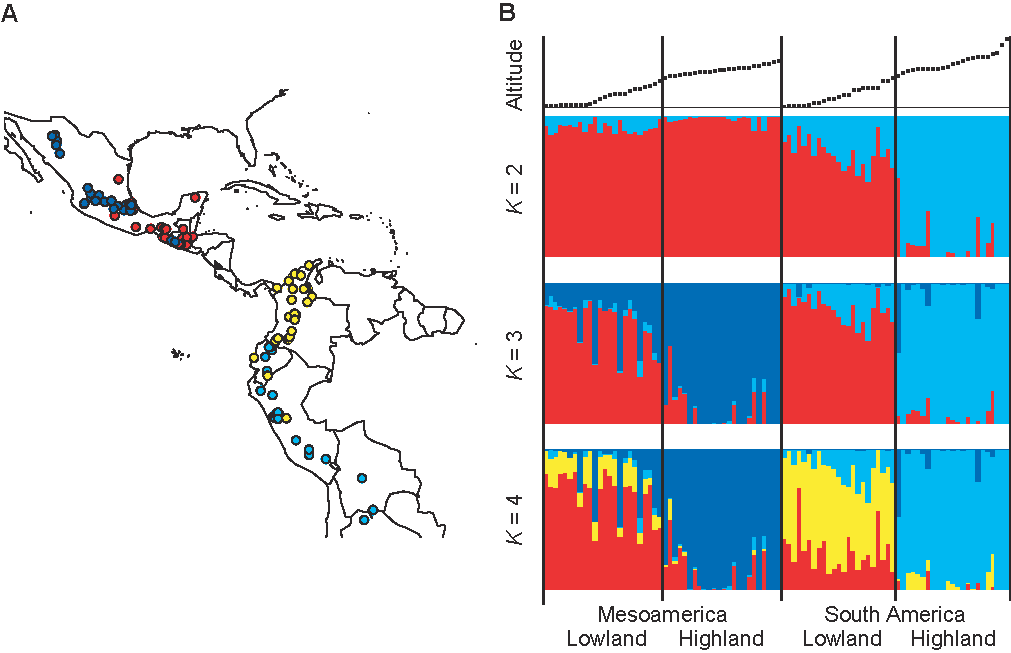
\includegraphics[width=0.8\textwidth]{fig/Fig2}
   \renewcommand{\baselinestretch}{0.9}
   \vspace{-3mm}
   \caption{(A) The sampling locations of landraces.  Red, blue, yellow and light blue dots represent Mexico lowland, Mexico highland, SA lowland and SA highland populations, respectively.  (B) The results of {\sf STRUCTURE} analysis with $K=2\sim4$.  The top panel shows the altitude of sampling locations of landraces, ranging from 0 to 4,000 m on the \emph{y}-axes.  The colors in $K=4$ correspond to those in panel (A).    }
\vspace{-6mm}
    \label{map}
  \end{center}
\end{figure*}
%%%%%%%%%%%%%%%%%%%%%%%%%%%%%%%%%%%%%%%%%% FIGURE


%%%%%%%%%%%%%%%%%%%%%%%%%%%%%%%%%%%%%%%%% FIGURE
\begin{figure*}[tb]   
  \begin{center}
   \vspace{-0mm}
   %\includegraphics[width=0.23\textwidth]{figs/model}
   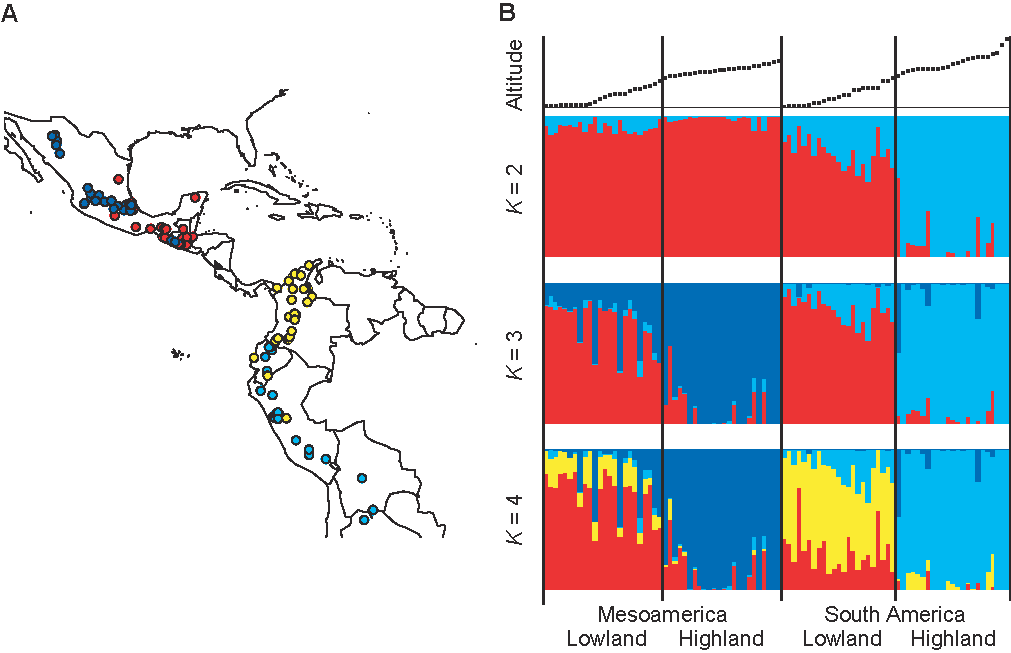
\includegraphics[width=0.8\textwidth]{fig/Fig2}
   \renewcommand{\baselinestretch}{0.9}
   \vspace{-3mm}
   \caption{(A) Sampling locations of landraces.  Red, blue, yellow and light blue dots represent Mexican lowland, Mexican highland, S. American lowland and S. American highland populations, respectively.  (B) Results of {\sf STRUCTURE} analysis of the maizeSNP50 SNPs with $K=2\sim4$.  The top panel shows the elevation, ranging from 0 to 4,000 m on the \emph{y}-axes.  The colors in $K=4$ correspond to those in panel (A).    }
\vspace{-6mm}
    \label{map}
  \end{center}
\end{figure*}
%%%%%%%%%%%%%%%%%%%%%%%%%%%%%%%%%%%%%%%%% FIGURE

\section*{Materials and Methods}

\subsection*{Materials and DNA extraction}
We included one individual from each of 94 open-pollinated landrace maize accessions from high and low elevation sites in Mexico and S. America (Table \ref{srkid}).   
Accessions were provided by the USDA germplasm repository or kindly donated by Major Goodman (North Carolina State University).  
Sampling locations are shown in Figure~\ref{map}A.  
Landraces sampled from elevations $<1,700$ m were considered lowland, while accessions from $>1,700$ m were considered highland.  
Seeds were germinated on filter paper following fungicide treatment and grown in standard potting mix.  
Leaf tips were harvested from plants at the five leaf stage.  
Following storage at $-80^{\circ}$C overnight, leaf tips were lyophilized for 48 hours.  
Tissue was then homogenized with a Mini-Beadbeater-8 (BioSpec Products, Inc., Bartlesville, OK, USA).  
DNA was extracted using a modified CTAB protocol \cite[]{CTAB}.  
The quality of DNA was ensured through inspection on a 2\% agarose gel and quantification of the ratio of light absorbance at 260 and 280 nm using a NanoDrop spectrophotometer (Thermo Scientific, NanoDrop Products, Wilmington, DE, USA).

\subsection*{SNP data}
We generated two complementary SNP data sets for the sampled maize landraces. 
The first set was generated using the Illumina MaizeSNP50 BeadChip platform, including 56,110 SNPs \cite[]{Ganal_2011_22174790}.  
SNPs were clustered with the default algorithm of the GenomeStudio Genotyping Module v1.0 (Illumina Inc., San Diego, CA, USA) and then visually inspected and manually adjusted.   
These data are referred to as "MaizeSNP50" hereafter.  
This array contains SNPs discovered in multiple ascertainment schemes \cite[]{Ganal_2011_22174790}, but the vast majority of SNPs come from polymorphisms distinguishing the maize inbred lines B73 and Mo17 (14,810 SNPs) or identified from sequencing 25 diverse maize inbred lines \cite[40,594 SNPs;][]{Gore20112009}.  

The second data set was generated for a subset of 87 of the landrace accessions (Table~\ref{srkid}) utilizing high-throughput Illumina sequencing data via genotyping-by-sequencing \cite[GBS;][]{Elshire2011}.
Genotypes were called using TASSEL-GBS \cite[]{Glaubitz_GBS} resulting in 2,848,284 SNPs with an average of 71.3\% missing data per individual.

To assess data quality, we compared genotypes at the 7,197 SNPs (229,937 genotypes, excluding missing data) that overlap between the MaizeSNP50 and GBS data sets. 
While only 0.8\% of 173,670  comparisons involving homozygous MaizeSNP50 genotypes differed in the GBS data, 88.6\% of 56,267 comparisons with MaizeSNP50 heterozygotes differed, nearly always being reported as a homozygote in GBS.
Despite this high heterozygote error rate,  the high correlation in allele frequencies between data sets ($r=0.89$; Figure~\ref{supp:correl_freq}) supports the utility of the GBS data set for estimating allele frequencies.  

We annotated SNPs using the filtered gene set from RefGen version 2 of the maize B73 genome sequence (\citealt{Schnable_2009_19965430}; release 5b.60) from maizesequence.org.  
We excluded genes annotated as transposable elements (84) and pseudogenes (323) from the filtered gene set, resulting in a total of 38,842 genes.

\subsection*{Structure analysis}
We performed a {\sf STRUCTURE} analysis \cite[]{Pritchard_2000_10835412,Falush_2003_12930761} using synonymous and noncoding SNPs from the MaizeSNP50 data. 
We randomly pruned SNPs closer than 10 kb and assumed free recombination between the remaining SNPs.
Alternative distances were tried with nearly identical results. 
We excluded SNPs in which the number of heterozygous individuals exceeded homozygotes and where the \emph{P}-value for departure from Hardy-Weinberg Equilibrium (HWE) using all individuals was smaller than 0.05 based on a \emph{G}-test. 
Following these data thinning measures, 17,013 biallelic SNPs remained. 
We conducted three replicate runs of {\sf STRUCTURE} using the correlated allele frequency model with admixture for \emph{K} = 2 through \emph{K} = 6 populations, a burn-in length of 50,000 iterations and a run length of 100,000 iterations. 
Results across replicates were nearly identical.

\subsection*{Demographic inference}
We tested three demographic models in which maize was differentiated into high- and lowland populations subsequent to domestication (Figure~\ref{model}). 
Observed joint frequency distributions (JFDs) were calculated using the GBS data set due to its lower level of ascertainment bias. 
A subset of synonymous and noncoding SNPs were utilized that had $\geq15$ individuals without missing data in both low- and highland populations and did not violate HWE.  
A HWE cut-off of $P<0.005$ was used for each subpopulation due to our under-calling of heterozygotes. 
In total, we included 18,745 synonymous and noncoding SNPs for the Mexican populations in Models IA and IB, 14,508 for the S. American populations in Model I and 11,305 for the Mexican lowland population and the S. American populations in Model II.  
We obtained similar results under more or less stringent thresholds for significance ($P < 0.05 \sim 0.0005$; data not shown), though the number of SNPs was very small at $P<0.05$.  
Demographic parameters were inferred with the software $\delta a \delta i$ \cite[]{Gutenkunst_2009_19851460}, which uses a diffusion method to calculate an expected JFD and evaluates the likelihood of the data using a multinomial assumption. 

%%%%%%%%%%%%%%%%%%%%%%%%%%%%%%%%%%%%%%%%% FIGURE
\begin{figure}[tb]   
  \begin{center}
   \vspace{-0mm}
   %\includegraphics[width=0.23\textwidth]{figs/model}
   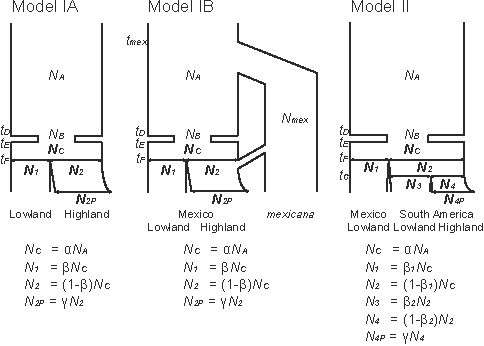
\includegraphics[width=0.5\textwidth]{fig/Fig3}
   \renewcommand{\baselinestretch}{0.9}
   \vspace{-3mm}
   \caption{ Demographic models of maize low- and highland populations.  Parameters in bold were estimated in this study.  See text for details.
   }
\vspace{-6mm}
    \label{model}
  \end{center}
\end{figure}
%%%%%%%%%%%%%%%%%%%%%%%%%%%%%%%%%%%%%%%%% FIGURE

\subsubsection{Model IA}
This model is applied to the Mexican and S. American populations.
We assume the ancestral diploid population representing \emph{parviglumis} follows a standard Wright-Fisher model with constant size.  
The size of the ancestral population is denoted by $N_A$.
At $t_D$ generations ago, the bottleneck event begins at domestication, and at $t_E$ generations ago, the bottleneck ends.  
The population size and duration of the bottleneck are denoted by $N_B$ and $t_B=t_D-t_E$, respectively.  
The population size recovers to $N_C=\alpha N_A$ in the lowlands.  
Then, the highland population is differentiated from the lowland population at $t_F$ generations ago.  
The size of the low- and highland populations at time $t_F$ is determined by a parameter $\beta$ such that the population is divided by $\beta N_C$ and $(1-\beta)N_C$.  
We assume that the population size in the lowlands is constant but that the highland population experiences exponential expansion after divergence: its current population size is $\gamma$ times larger than that at $t_F$. \\

%jri{isn't this really a shrinking population in the lowlands, since $\beta N_C<N_C$ ? wouldn't we want instead for lowlands to stay at $N_C$ and a new population branching off?  how much do we worry about this?}
%\st{actually, our conclusion holds when I assumed the pop size of lowlands stays at $N_C$.  However, the likelihood is a bit better in my original model.}

\subsubsection{Model IB}
We expand Model IA for the Mexican populations by incorporating admixture from the teosinte \emph{mexicana} to the highland Mexican maize population.  
The time of differentiation between \emph{parviglumis} and \emph{mexicana} occurs at $t_{mex}$ generations ago.  
The \emph{mexicana} population size is assumed to be constant at $N_{mex}$.  
At $t_F$ generations ago, the Mexican highland population is derived from admixture between the Mexican lowland population and a portion $P_{mex}$ from the teosinte \emph{mexicana}.\\  

\subsubsection{Model II}
The final model includes the Mexican lowland, S. American lowland and highland populations.  
This model was used for simulating SNPs with ascertainment bias (see below).  
At time $t_F$, the Mexican and S. American lowland populations are differentiated, and the sizes of populations after splitting are determined by $\beta_1$.  
At time $t_G$, the S. American lowland and highland populations are differentiated, and the sizes of populations at this time are determined by $\beta_2$.  
As in Model IA, the S. American highland population is assumed to experience population growth with the parameter $\gamma$.\\

Estimates of a number of our model parameters were available from previous work.    
$N_A$ was set to 150,000 using estimates of the composite parameter $4N_A\mu \sim 0.018$ from \emph{parviglumis}  \cite[]{Eyre-Walker_1998_9539756,Tenaillon_2001_11470895,Tenaillon_2004_15014173,Wright_2005_15919994,Ross-Ibarra_2009_19153259} and an estimate of the mutation rate $\mu \sim 3\times 10^{-8}$ \cite[]{Clark_2005_16079248} per site per generation.  
The severity of the domestication bottleneck is represented by $k=N_B/t_B$ \cite[]{Eyre-Walker_1998_9539756,Wright_2005_15919994}, and following \cite{Wright_2005_15919994} we assumed $k=2.45$ and $t_B=1,000$ generations.  
Taking into account archaeological evidence \cite[]{Piperno_2009_19307570}, we assume $t_D=9,000$ and $t_E=8,000$.  
We further assumed $t_F=6,000$ for Mexican populations in Models IA and IB \cite[]{Piperno_2006_69}, $t_F=4,000$ for S. American populations in Model IA \cite[]{Perry_2006_16511492,Grobman_2012_22307642}, and $t_{mex}=60,000$, $N_{mex}=160,000$ \cite[]{Ross-Ibarra_2009_19153259}, and $P_{mex}=0.2$ \cite[]{vanHeerwaarden_2011_21189301} for Model IB. 
For both Models IA and IB, we inferred three parameters ($\alpha$, $\beta$ and $\gamma$), and, for Model II, we fixed $t_F=6,000$ and $t_G=4,000$ \cite[]{Piperno_2006_69,Perry_2006_16511492,Grobman_2012_22307642}  and estimated the remaining four parameters ($\alpha$, $\beta_1$, $\beta_2$ and $\gamma$).

\subsection*{Population differentiation}
We used our inferred demographic model to generate a null distribution of $F_{ST}$.
As implemented in $\delta a \delta i$ \cite[]{Gutenkunst_2009_19851460}, we calculated an expected JFD given estimated demographic parameters and the sample sizes from our highland and lowland populations.
Then, we converted the JFD into the distribution of $F_{ST}$ values.
The \emph{P}-value of a SNP was calculated by $P(F_{ST\_E}\geq F_{ST\_O}|p\pm 0.05) = P(F_{ST\_E}\geq F_{ST\_O} \cap p\pm 0.05)/P(p\pm 0.05)$, 
where $F_{ST\_O}$ and $F_{ST\_E}$ are observed and expected $F_{ST}$ values and $p\pm 0.05$ is the set of loci with mean allele frequencies within 0.05 of the mean allele frequency of the SNP across both highland and lowland populations.

Generating the null distribution of differentiation for the MaizeSNP50 data requires accounting for ascertainment bias. 
Evaluation of genetic clustering in our data (not shown) coincides with previous work \cite[]{Hufford_2012_22660546} in suggesting that the two inbred lines most important in the ascertainment panel (B73 and Mo17) are most closely related to Mexican lowland maize.  
We thus added two additional individuals to the Mexican lowland population and generated our null distribution using only SNPs for which the two individuals had different alleles.
For model IA in S. America we added two individuals at time $t_F$ to the ancestral population of the S. American lowland and highland populations because the Mexican lowland population was not incorporated into this model. 
For each combination of sample sizes in lowland and highland populations, we generated a JFD from $10^7$  SNPs using the software {\sf ms} \cite[]{Hudson_2002_11847089}.
Then, we calculated \emph{P}-values from the JFD in the same way.
We calculated $F_{ST}$ values for all SNPs that had $\geq10$ individuals with no missing data in all four populations and showed no departure from HWE at the 0.5\% (GBS) or 5\% (MaizeSNP50) level. 

%\jri{we don't correct for allele frequency (or heterozygosity) in our Fst outlier analysis do we?  if not, this is a problem I think.}
%\st{I did.  No essential change}

%\jri{do we use all GBS data in the Fst outlier test, or just silent SNPs? we should be able to use nonsynonymous too, right?}
%\st{I used all.}

\subsection*{Haplotype sharing test}
We performed a \underline{p}airwise \underline{h}aplotype \underline{s}haring (PHS) test to detect further evidence of selection, following \cite{Toomajian_2006_16623598}.  
To conduct this test, we first imputed and phased the combined SNP data (both GBS and MaizeSNP50) using the {\sf fastPHASE} software version 1.4.0 \cite[]{Scheet_2006_16532393}.  
As a reference for phasing, we used data (excluding heterozygous SNPs) from an Americas-wide sample of 23 partially inbred landraces from the Hapmap v2 data set  \cite[]{Chia_2012_22660545}.  
We ran {\sf fastPHASE}  with default parameter settings.  
PHS was calculated for an allele \emph{A} at position $x$ by

\begin{equation}
  \label{phs-1}
  \begin{array}{l}
  \displaystyle{
PHS_{x_A} = \sum^{p-1}_{i=1}\sum^{p}_{j=i+1}Z_{ijx}  / \Bigl( \begin{array}{c} p \\ 2 \\ \end{array} \Bigr) 
- \sum^{n-1}_{i=1}\sum^{n}_{j=i+1}Z_{ijx}  / \Bigl( \begin{array}{c} n \\ 2 \\ \end{array} \Bigr) 
  }
  \end {array} 
  \textrm{,}
\end{equation}
\noindent where $n$ is the sample size of haploids, $p$  is the number of haploids carrying the allele $A$ at position $x$, and

\begin{equation}
  \label{phs-2}
  \begin{array}{l}
  \displaystyle{
Z_{ijx} = \frac{ d_{ijx} - \bar{d_{ij}} }{ \sigma_{ij} }
  }
  \end {array} 
  \textrm{,}
\end{equation}
\noindent where $d_{ijx}$ is the genetic distance over which individuals $i$ and $j$ are identical surrounding position $x$, $\bar{d_{ij}}$ is the genome-wide mean of distances over which individuals are identical, and $\sigma_{ij}$ is the standard deviation of the distribution of distances.  
The \emph{P}-value for each allele was calculated as the proportion of alleles of the same frequency genome-wide that have a larger PHS value. 

Genetic distances were obtained for the MaizeSNP50 data \cite[]{Ganal_2011_22174790} and fit using a tenth degree polynomial curve to all SNPs (data not shown).
 
%%%% PLR:
\subsection*{Theoretical evaluation of convergent evolution }
We build on results from \cite[]{ralph2014convergent} to assess whether the abundance and degree of coincidence of presumably adaptive high-$F_{ST}$ alleles is consistent with what is known about the population history of maize, we evaluated the rate at which we expect an allele that provides a selective advantage at higher elevation to arise by new mutation in a highland region ($\mutrate$), and the rate at which such an allele already present in the Mexican highlands would transit the intervening lowlands and fix in the Andean highlands ($\migrate$).
% We suggest below that many of the high-$F_{ST}$ alleles are locally adaptive, and the degree of coincidence between highland regions informs us about whether these adaptations occurred convergently, or if alleles were transmitted between the two by migration. 
We assume alleles adapted in the highlands are slightly deleterious at lower elevation, consistent with empirical findings in reciprocal transplant experiments in Mexico \cite[]{Mercer2008}.
These numbers depend most strongly on the population density, the selection coefficient, and the rate at which seed is transported long distances and replanted.
To obtain specific predictions, we computed $\mutrate$ and $\migrate$ at various parameter values.
We also checked these with simulations and more detailed computations, described in the Appendix.
Here we describe the mathematical details; readers may skip to the results without loss of continuity.\\

%To calculate the rate at which new mutations appear and fix in a highland population, $\mutrate$, we multiplied the total population size of the highlands by the mutation rate per generation.
\subsubsection{Demographic model}
Throughout, we followed \citet{vanHeerwaarden2010} in constructing a detailed demographic model for domesticated maize.
We assume fields of $N=10^5$ plants are replanted each year from $N_f=561$ ears, either from completely new stock (with probability $p_e=0.068$), from partially new stock (a proportion $r_m=0.2$ with probability $p_m=0.02$), or  otherwise entirely from the same field.
Each plant is seed parent to all kernels of its own ears, but can be pollen parent to kernels in many other ears; a proportion $m_g=0.0083$ of the pollen-parent kernels are in other fields.
Wild-type plants have an average of $\mu_E=3$ ears per plant, and ears have an average of $N/N_f$ kernels; each of these numbers are Poisson distributed.
The mean number of pollen-parent kernels, and the mean number of kernels per ear, is assumed to be $(1+s_b)$ times larger for individuals heterozygous for the selected allele.
Migration is mediated by seed exchange -- when fields are replanted, the seed is chosen from a random distance away with mean $\sigma_s=50$km, but plants only pollinate other plants belonging to the same village (distance 0).
Each individual can have offspring in three categories: local seed, local pollen, and migrant seed; the mean numbers of each of these are determined by the condition that the population is stable (i.e. wild-type, diploid individuals have on average 2 offspring) except that heterozygotes have on average $(1+s_b)$ offspring that carry the selected allele.
Each ear has a small chance of being chosen for replanting, so the number of ears replanted of a given individual is Poisson, and assuming that pollen is well-mixed, the number of pollen-parent kernels is Poisson as well.
Each of these numbers of offspring has a mean that depends on whether the field is replanted with new stock, and whether ears are chosen from this field to replant other fields, so the total number of offspring is actually a mixture of Poissons; these means, and more details of the computations, are found in Appendix \ref{apx:demographic_model}.
At these parameter values, we compute that the variance in number of offspring, $\xi^2$, is between 20 (for wild-type) and 30 (for $s_b=0.1$), and the dispersal distance (mean distance between parent and offspring) is $\sigma=1.8$km.\\

\subsubsection{New mutations}
The rate at which new mutations appear and fix in a highland population, which we denote $\mutrate$, is equal to the total population size of the highlands multiplied by the mutation rate per generation and by the chance that a single such mutation successfully fixes (i.e.\ is not lost to drift).
The probability that a single new mutant allele providing benefit $s_b$ to heterozygotes at high elevation will fix locally in the high elevation population is approximately $2s_b$ divided by the variance in offspring number \citep{jagers1975branching}.
The calculation above is not quite correct, as it neglects migration across the altitudinal gradient, but exact numerical calculation of the chance of fixation of a mutation as a function of the location where it first appears indicates that the approximation is quite good (see Figure~\ref{sfig:prob_estab}); for theoretical treatment see \citet{pollak1966survival} or \citet{barton1987establishment}.

 %\plr{could alternatively: (a) describe the math; or (b) cut this down further.}
 %I actually like this as is, but think we should expand math as separate appendix. my thinking is math will be of interest to a subset of audience, so perhaps best presented fully but at end. thoughts?
 %\plr{added a signpost for non-mathey readers to skip this at the start}

Concretely, the probability that a new mutation destined for fixation will arise in a patch of high-elevation habitat of area $A$ in a given generation is a function of the density of maize per unit area $\rho$, the selective benefit $s_b$ it provides, the mutation rate $\mu$, and the variance in offspring number $\xi^2$.
In terms of these parameters, the rate of appearance is 
\begin{align} \label{eqn:mutrate}
  \mutrate = \frac{2 \mu \rho A s_b}{\xi^2} .
\end{align}

\subsubsection{Migration}
A corresponding expression for the chance that an allele moves from one highland population to another is harder to intuit, and is addressed in more depth in \citep{ralph2014convergent}.
If an allele is beneficial at high elevation and fixed in the Mexican highlands but is deleterious at low elevations, then at equilibrium it will be present at low frequency at migration-selection balance \citep{slatkin1973geneflow} in nearby lowland populations.
This equilibrium frequency decays exponentially with distance, so that the highland allele is present at distance $R$ from the highlands at frequency $C \exp(- R \sqrt{2s_m} / \sigma)$, where $s_m$ is the deleterious selection coefficient for the allele in low elevation, $\sigma$ is the mean dispersal distance, and $C$ is a constant depending on geography ($C\approx 1/2$ is close).
Multiplying this frequency by a population size gets the predicted number (average density across a large number of generations) of individuals carrying the allele.
Therefore, in a lowland population of size $N$ at distance $R$ from the highlands, $(N/2)  \exp(- R \sqrt{2s_m} / \sigma)$ is equal to the probability that there are any highland alleles present, multiplied by the expected number of these given that some are present.
Since the latter is at least 1, this puts an upper bound on the rate of migration
%the chance there are any present in a given generation is no more than $(N/2) \exp(- R \sqrt{2s_m} / \sigma)$, and so this puts an upper bound on $\migrate$.
%Therefore, we would need to wait $\Tmig = (2/N)\exp(R \sqrt{2s_m} / \sigma)$ generations for a rare such excursion to occur.
%In other words, we can bound the rate of migration by
\begin{align}
  \migrate \le (N/2)  \exp(- R \sqrt{2s_m} / \sigma),
\end{align}
and we we would need to wait $\Tmig = 1/\migrate$ generations for a rare such excursion to occur.
%with $N$ being the total size of the unadapted highland population, and $R$ the distance from the adapted to the yet-unadapted highland populations.
This calculation omits the probability that such an allele fixes ($\approx 2s_b/\xi^2$), but since such alleles arrive by migration, this omission is unlikely a large effect and is conservative.








\intpu{results}

\section*{Conclusions}
1. We successfully inferred demography and detected the candidates of adaptive loci to highland climates in Mexico and South America by utilizing GBS and 55-k chip.

2. The main conclusion is parallel adaptation is rare in maize highland adaptation.


\begin{acknowledgments}
  We appreciate the helpful comments of P. Morrell and the members of Ross-Ibarra lab and Coop labs.   
%add in formal acknowledgement of USDA. use grant number from Joost's 2012 PNAS paper.
\end{acknowledgments}


%Note that a SNP with significant \emph{P} value is not necessarily the causative variant because we cannot rule out the possibility that the SNP is just linked to the true causative one.  

%, or the two SNPs are linked to the causative SNPs and recombination .

%    The distance of genetic units would be fairly long, compared to the rapid decay of linkage disequilibrium in maize (roughly 100 bp; Supp Fig. X) \cite[]{Tenaillon_2001_11470895}.  We just assumed that SNPs within a genetic unit have the same functional effect or link to the functional SNP, and based on this assumption, we screened SNPs showing Pattern C of parallel adaptation in Fig.~\ref{fig1}.  \textcolor{red}{Do you have a better idea?}  \jri{i like this but i think we need to be more explicit about relating our analyses back to the patterns.  are we doing this because of linkage or because of biology or both?} \mbh{It might be a good idea to mention linkage to the heuristic set up in Figure 1} 

% \jri{ so this is worth thinking about.  what do we call it if the same SNP was selected but in alternate directions?  i think you need to explain "recombination" further.  i assume you mean that both snp alleles occurred on some background that was then selected in parallel?  since we don't know what SNP was selected how do we categorize this?  Also, somewhere we need to make clear that our different models of parallel adaptation assume that if we see high $F_{ST}$ in two pops that it's because that snp is selected for.  It's just as possible to have the same SNP allele selected in both pops but because it was on different backgrounds! }

% \textcolor{red}{Parallel adaptation in lowland populations also occurred!!} \jri{ not sure how we know this was parallel adaptation in lowland... could be ancestral snp on a derived background (recombination), could be the ancestral allele is suddenly beneficial in a highland habitat (parallel adaptation in highland) or that the new derived allele is beneficial in lowland (parallel adaptation in lowland).  can we distinguish among these (or other) options? }

%Note that the result was not changed when using working gene set. 
%\jri{need to add working gene set not changing result into text.}

%A lot of adaptive SNPs are from standing variation.  That was confirmed by SNPs of teosinte in Hapmap v2. 

%\jri{is standing variation defined in teosinte or should it be defined in lowland ancestral pop? some SNPs that are monomorphic in teo might have been polymorphic in lowland ancestor? } \mbh {It seems if we're talking about highland adaptation from standing variation, it has to be from variation in lowland maize}





%\subsection*{Check overlap with QTL regions} \jri{ skip both these for now}

%\subsection*{Maize cys}
















\bibliography{MZpara1,MZpara2,plr-hilo}
\bibliographystyle{geneticsT2}

\end{document}





%%%%%%%%%%%%%%%%%%%%%%%%%%%%%%%%%%%%%%%%%%%%%%%%%%%%%%%%%%%%
\renewcommand{\arraystretch}{1.1}
\begin{table}[tb]

\begin{center}
 \caption[]{Parallel adaptation\hspace*{0.3cm}}
  \textbf{}\\[-2mm]
{\fontsize{7}{11}\sf
    \begin{tabular}{lllcccccl} \hline
       & & \\[-3mm]
     Description  & Number of genetic units\\[0.1cm]
    \hline
Pattern A or B     & 45 \\
Pattern C from standing variation & 16\\ 
Pattern C from standing variation and & 2\\
\ \ vi new mutations & \\
Total & 63\\[1mm]
    \hline
  \multicolumn{2}{l}{$^{a}$ \textcolor{red}{In this table, I did not use the information of teosinte polymorphisms.}}\\
    \end{tabular}
    \label{paraGU}  % caption is needed to make this work
}
\end{center}
\end{table}
\renewcommand{\arraystretch}{1}
%%%%%%%%%%%%%%%%%%%%%%%%%%%%%%%%%%%%%%%%%%%%%%%%%%%%%%%%%%%%


% pre
%%%%%%%%%%%%%%%%%%%%%%%%%%%%%%%%%%%%%%%%%%%%%%%%%%%%%%%%%%%%
\renewcommand{\arraystretch}{1.1}
\begin{table}[tb]

\begin{center}
 \caption[]{Parallel adaptation\hspace*{0.3cm}}
  \textbf{}\\[-2mm]
{\fontsize{7}{11}\sf
    \begin{tabular}{lllcccccl} \hline
       & & \\[-3mm]
     Description  & Number of genetic units\\[0.1cm]
    \hline
Parallel adaptation     &  \\
Pattern A or B     & 45 \\
Pattern C from standing variation & 16\\ 
Pattern C from standing variation and & 2\\
\ \ vi new mutations & \\
Total & 63\\
      \hline
    & & \\[-3mm]
Only Mexico     &  \\
From standing variation & 635 \\
New mutations & 65 \\
Both mechanisms & 16 \\
Total & 716\\
      \hline
    & & \\[-3mm]
Only South America     &  \\
From standing variation & 458 \\
New mutations & 36 \\
Both mechanisms & 4 \\
Total & 498\\[1mm]
    \hline
  \multicolumn{2}{l}{$^{a}$ \textcolor{red}{Check teosinte polymorphisms on Hapmap2 later.}}\\
    \end{tabular}
    \label{paraGU}  % caption is needed to make this work
}
\end{center}
\end{table}
\renewcommand{\arraystretch}{1}
%%%%%%%%%%%%%%%%%%%%%%%%%%%%%%%%%%%%%%%%%%%%%%%%%%%%%%%%%%%%

